% % !TeX spellcheck = en_GB
\begin{wrapfigure}{r}{0.44\textwidth}
	%	\vspace{-\normalbaselineskip}
	\centering
	\begin{subfigure}[b]{0.4\textwidth}
		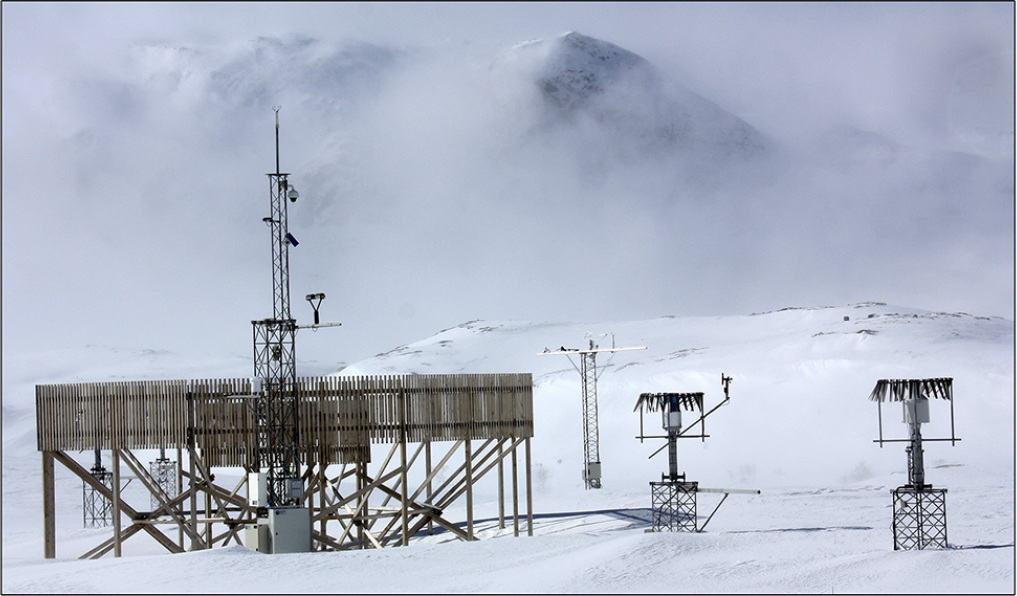
\includegraphics[width=\textwidth]{./fig_instruments/Dofe.png}
		\caption{}\label{fig:Dofe}
	\end{subfigure}
	\begin{subfigure}[b]{0.4\textwidth}
		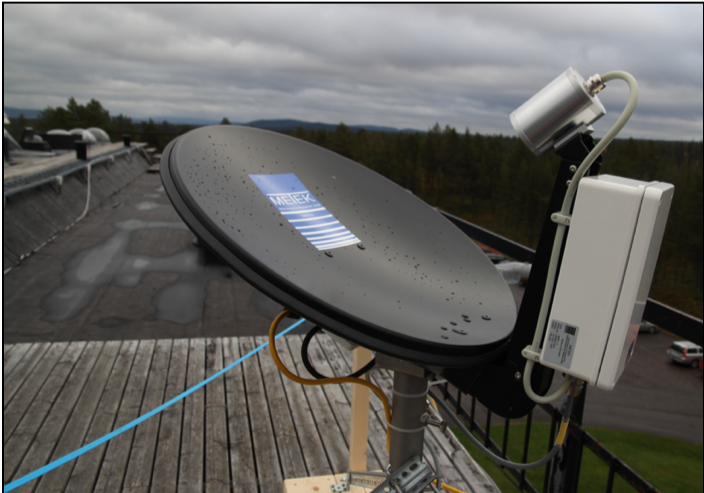
\includegraphics[width=\textwidth]{./fig_instruments/MRR.png}
		\caption{}\label{fig:MRR}
	\end{subfigure}
	\begin{subfigure}[b]{0.4\textwidth}
		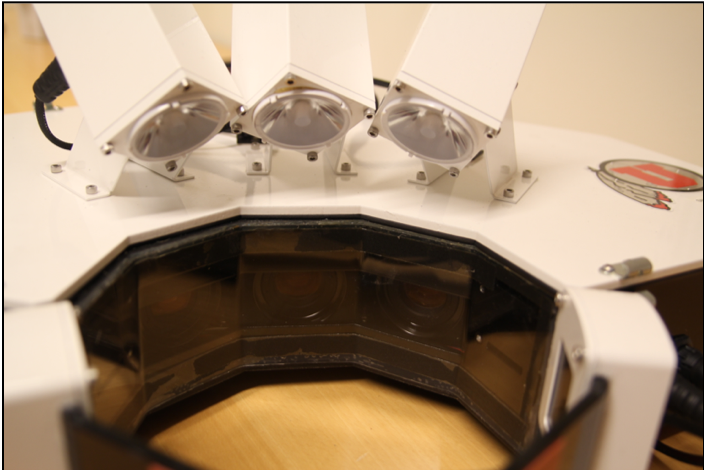
\includegraphics[width=\textwidth]{./fig_instruments/MASC.png}
	\end{subfigure}	
	\begin{subfigure}[b]{0.4\textwidth}
		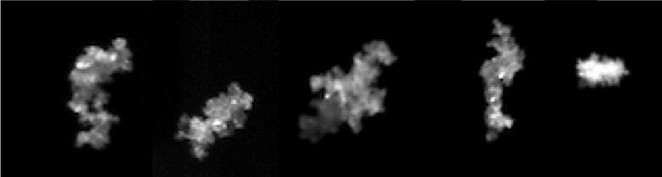
\includegraphics[width=\textwidth]{./fig_instruments/MASC_snowflakes.png}
		\caption{}\label{fig:MASC}
	\end{subfigure}	
	\caption{\protect\subref{fig:Dofe}: Double fence and unprotected precipitation gauges at Haukeliseter, from \cite{wolff_derivation_2015}. \protect\subref{fig:MRR}: Micro Rain Radar. \protect\subref{fig:MASC}: MASC and images taken by instrument. \textcolor{red}{Lower panel taken from \cite{cooper_variational_2017} maybe we get one for Haukeli?}}
	\vspace{-\normalbaselineskip}
\end{wrapfigure}
